
\section{Motivation} \label{sec:motivation}

\subsection{Heterogeneous Graphs}

Graph Neural Networks (GNNs) have been successfully employed for many tasks~\cite{wang_embeddings_2022}.
Many of the early results only work on homogeneous graphs, however real-world data is often heterogeneous.
For example, in the Open Academic Graph (OAG), nodes for \emph{papers} and nodes for \emph{authors} are fundamentally different,
and should be treated as such.


% D.
% I really ain't a fan of heavy-handed math right upfront. That really blocks the flow. We don't need all this formalism. We should keep the degree of formalization low, bring our point across with a quite intuitive language, as in the proposal of Nebi's Msc. thesis or all other posts/reports.
% I would go as far as to say that unnecessary formalization is a way to protect oneself behind a curtain (shroud) of complexity. You don't invite people in, you keep them away. So, it's not a social form of writing and writing is designed to be social (especially when writing for a broad public as in a report; not when writing in chat where the form almost takes on almost a journal aspect).
% Use natural language and let the reader fill the dots of the low-level patterns. My go-to example of how excellent maths hardly use any math. notation: [An introduction to compressive sampling](https://authors.library.caltech.edu/10092/1/CANieeespm08.pdf)
% 

The challenge of a GNN is to embed the nodes and edges in such a way as to deliver good performance on a variety of downstream tasks, e.g. classifying new nodes or providing recommendations.

% intro of HGT; bigger framework
One solution for this has been the Heterogeneous Graph Transformer (HGT)~\cite{hu2020heterogeneous}, 
where each embedded node learns a message function and an aggregation function, and at each step computes a message for each of its neighbours and aggregates the messages it receives from its neighbours based on an attention mechanism.

One major advantage of HGT over previous GNNs has been the usage of the heterogeneity of graphs.
That is, the nodes and edges in the graph can be of different \emph{types}.
For example, when looking at a graph of academic works some nodes might be of the type \emph{author} while others are of the type \emph{paper}.
HGT learns different models for each type.
This leads to performance improvements, but can only be leveraged if the types in the graph are labeled and the graph is ``sufficiently heterogeneous'', i.e. there is not one single type that (nearly) all nodes or edges belong to.


%% DONE? 
% D.
% I get lost in details.
% Why do we do all this? Bunch of math thrown at me (by "me" I mean a standard reader; I understand all this math just fine, but I'm speaking when I put myself in their shoes).
% The problem has to be stated. I have to be interested, i.e., the text has to raise my interest. And only then will I be willing to go through the math. And I'll understand in what context I am seeing the math and that'll allow me to understand the math quickly.
% It's just like you don't want to present code before you presented the high-level architecture of a code base. Once sb. understands the high-level interaction among components, they are able to place any piece of code they see in this broader scheme.
% Here, in math, we need to make our reader get the big picture of how communication happens, illustrated in a way that takes little time and effort to capture intuitively, as with [HGT](https://dl.acm.org/doi/pdf/10.1145/3366423.3380027), _Fig. 2_, and then we can speak about going lower-level. Or, actually, I would only go lower-level in a formalization chapter after the intro chapter. See how this math-heavy paper introduces their math: [Massively parallel algorithms for personalized pagerank](https://dl.acm.org/doi/pdf/10.14778/3461535.3461554), _Introduction_. It's just sprinkled in the text, flowing with the natural language. And they wait until their second section, _Preliminaries_, to lay out more mathematical structure with theorems and definitions. And anything that would be really painful to read, like a proof, that would normally go into the appendix because it brings low conceptual value for the effort put into it to read it (and to write it), i.e., explains only little how things work, and what the intuition behind it is, "teach" not very efficiently, if you will.
% 
% So, I understand where you come from, namely from math courses where there is zero motivation and only definitions and the audience is forced to follow tenuously until they grasp the material well and then the audience is finally allowed to use the framework they learned and as they use it they finally understand what the framework is for... but this academic form of presenting the content is a very inefficient form of knowledge transfer:
% - the audience is lost upfront; there is no uninterrupted common thread from motivation to problem to solution (as in [SC2 paper](https://paperpile.com/shared/ymOJNB), for example). And so people cannot just read end-to-end
% - the standard math-course-like format really does not support random access / gradual reading. Normally, there is an intuitive and accessible high-level presentation of the concept in the abstract and less so in the introduction (or, e.g., as I give to my prof. in [eval_theses](https://drive.google.com/open?id=1NRpu3LJdph71ax0NyZ0Itb4re6APUEGC&authuser=adastruct%40gmail.com&usp=drive_fs)). And this introduction serves as an index and people can jump to different parts, pseudo-code, software design, experiments, and be able to understand them – esp. people well versed in the field. See [The Writing Corner]https://adastruct.slack.com/archives/C0207JY553J/p1644423270924359?thread_ts=1644423270.924359) for more. And for this to work, the reader has to be eased into the content, from intuitive in the introduction (aka the proposal; it's the same in tone) to geeky in chapter deeper down.
% 
% ->
% Please move the geeky formalization away from the proposal to a new first chapter, "preliminaries", which we won't be using in the proposal but will be using in the thesis.
% Please write the motivation in a more acessible manner; the why, the what's done out there and why there is a gap, taking a path from [HGT](https://dl.acm.org/doi/abs/10.1145/3366423.3380027) through [Few-Shot](https://arxiv.org/pdf/1711.04043) or similar to the problem we're trying to solve.
% 


\subsection{Prior attempts at dealing with insufficient heterogeneity}
%% TODO expand
% D.
% ok, presentation of gap here
% Can we just get rid of the math from before and only leave this paragraph and say this paragraph does a good job of presenting the gap already?
% Nah. This paragraph would have to be extended into a larger structure of own paragraphs, though.
% 
% 


There have been some attempts at dealing with insufficiently heterogeneous graphs in the past.

\paragraph{Heterogeneous Graph Structure Learning}$\,$

Heterogeneous Graph Structure Learning (HGSL)~\cite{zhao_heterogeneous_2021} generates a new \emph{relation subgraph} based on the original graph, and then uses that one for downstream tasks.
The relation subgraph is created by fusing a \emph{feature graph} $S^{Feat}$, and a \emph{semantic graph} $S^{Sem}$
with the original graph $A$, and then using a GNN of your choice on the new graph $A'$.
The feature (similarity) graph evaluates the probability of the existence of an edge with a given type between two
nodes based on node features, and the semantic graph is based on the higher-order topology of the graph.

While this produces good results, it adds a time complexity of $O(|\mathcal{V}|^2 + |\mathcal{R}|)$ to the training, making it infeasible for sufficiently large graphs, and the found additional heterogeneous structure in the new graph $A'$ is completely uninterpretable to humans.

\paragraph{Super Nodes}$\,$

Another attempt have been Super~Nodes~\cite{stanley_compressing_2018}. 
In an $N$-node network, Super Nodes work by selecting $S << N$ seed nodes,
and then agglomerating the remaining $N-S$ nodes around the seeds to create super nodes.
Then the $S$-node network gets fed into Community~Detection~\cite{fortunato_community_2010}.
The agglomeration works by minimizing the \emph{under segmentation error} $U$:
Let $N$ be the number of nodes, $K$ be the number of communities $\{k_1 , \dots , k_K\}$, and $S$ be the number of
super nodes $\{s_1 , \dots , s_S \}$. Then Super~Nodes minimizes:

\[ U = \frac{1}{K} \sum_{i=1}^{K} \frac{ [ \sum_{s_j | s_j \cap k_i \not= \varnothing } |s_j | ] - |k_i |}{|k_i|} \]

This is efficient and produces good results. It is also interpretable: the super nodes could be seen as new ``types'' in the graph, with their corresponding seed nodes being representative of their type.

However, these new types are not treated qualitatively differently.
All different super nodes are still treated via the same algorithm.
A truly heterogeneous treatment of the newly found types would need additional parameters for each type, while Super~Nodes just compresses nearby similar regions of the graph into one node that is still treated the same as the rest.

Additionally, Super~Nodes is tied to Community~Detection, and cannot easily be used with arbitrary graph algorithms.

While a number of other graph compression algorithms have since been developed~\cite{besta_survey_2019}, all of them are also plagued by the first problem.
%% TODO
% D.
% > DONE? Mentioned that super nodes cannot easily work together with others and put MAML into next steps
% 
% Ok, but then saying in the solution we do a tree is selling ourselves short.
% The solution should contain all the parts we want to deliver.
% solution = prototype + next steps (or next steps = solution - prototype), as I wrote in [Writing – Examples](https://adastruct.slack.com/archives/C0207JY553J/p1644667640995319?thread_ts=1644423270.924359&cid=C0207JY553J), _Solution vs. Prototype vs. Next Steps_
% and so there should be nothing in the next steps that's not already in the solution
% 
% solution = [Organic Meta](https://adastruct.slack.com/archives/C022U4MU8BV/p1682343482796529?thread_ts=1682343422.127599&cid=C022U4MU8BV)
% 
% The point is that then we can reuse the solution as is in the final thesis (up to some changes to adapt to what we actually delivered), be it in the solution, or, extended, in the solution design chapter. The format of the proposal is so as to minimize the extra work later.
% 


\section{Problem Statement} \label{sec:problem_statement}
The advances of heterogeneity are only applicable if the data is heterogeneous and labeled as such, and if the types are sufficiently diverse.

Hence, we propose to address the following problem:
% 
\emph{How to find and process types or subtypes in a (near-)homogeneous graph?}

%% TODO reformulate
% D.
% "types or subtypes" = internal language, not understandable to the outside.
% I would rather say models at all times. That avoids us getting lost in sub-, super-, whatever. And nodes are in relation with other nodes and the relation allow them to borrow models from other nodes.
% 



\section{Solution} \label{sec:solution}

%\paragraph{Subtypes}$\,$

To organically extract and model heterogeneity, we introduce a new set of \emph{subtypes}.

These can be seen as a directed acyclic graph of types.
Each node in the type graph represents a type in the original graph, and computes an ``importance'' of that type,
which represents the current difficulty of modeling that type.
That is, the higher the error for items of a certain type, the higher its importance will be.
Once the importance of a type reaches a certain threshhold, we split the type into subtypes.
%% DONE?
% D.
% > In practice, we implement this as a tree of types.
% 
% No? We said we can do a graph of models instead.
% = [Organic Meta](https://adastruct.slack.com/archives/C022U4MU8BV/p1682343482796529?thread_ts=1682343422.127599&cid=C022U4MU8BV)
% 
% D.
% "Each time we want to split a type into subtypes"
% When do we declare we need to split a type into subtypes?
% 
% D.
% "In practice, we implement this as a tree of types."
% also, we're not trying to present the practice, the actual implementation. We're trying to present the general framework.
%

We train a separate model for classifying nodes into types which is then applied when splitting.
% = reactive clustering
Each node in the type graph has its own model, and the nodes of the graph are processed by going through each corresponding model from the bottom up.
This way, each subtype both shares parameters with all of its supertypes, as all of the models above are applied,
and also has its own set of parameters to specialise.

%% TODO
% D.
% The tree using tentative clustering would be only a prototype because it's restrictive in its functionalities and scope; it's a proof of concept.
% 
% D.
% ### Solution: Differential Meta
% _Borrowing another Model: "Subtyping"_
% The subtyping should instead consist of a node's model being the aggregate of models from other nodes, applied to the state to create the model so that we can increase/reduce the level of meta. That's like going deeper in a neural network.
% 
% _Searching for new Models_
% = projection using key, query, value of a node for the models, to compute the affinity with other nodes nearby to borrow their model.
% 
% _Searching for new Models_
% - When to decide to create a new node as a new model (= what we called subtyping)
% - When to decide to search for a new node as a model to borrow
% = driven by meta-agents, from @Hassan or @Fabian
% 
% _Aggregation of Models_
% Key, query, value applied on the different models borrowed and summed up, as in Transformers.
% -> includes the classic subtyping as special case, namely when we force the key, query, value to fully borrow weights from one node vs. weights from another, and we ignore the node state: f:x -> f.
% 
% _State Encoding_
% State observed = a value passed through models.
% 
% _State Update_
% key, query, value updated as part of the state
% the model gets updated when used; the update propagates back, changing state and models used.
% 
% All propagation and search happens lazily. That is, if a node considers there is nothing to tell other nodes, it shouldn't propagate/search/etc.
% Laziness to get from #dynamic_metagraphs, esp. from @Marcel Längrich, as a step further in the kNN story.
% 
% 
% Please use a language abstract like this to present the solution, of general patterns. Not of specific methods.
% 


\section{Contributions}

Our contributions are as follows.

\subsection{Find types in a previously homogeneous graph} 
For example, given a set of images to classify with classes such as "Dog", "Cat", "Car", or "Motorcycle",
our approach might first class the images into types like "Animal" and "Vehicle", and then classify based on that.

\subsection{Find specialisations in large groups of single types} 
For example, in the OAG dataset it might be beneficial to further specify a type like "paper" into something like "machine-learning paper" to improve performance.

\subsection{Find different, perhaps better suited type classifications} 
By erasing the previously annotated types and finding new ones, the network has more control over how to approach a given node.
For example, in the OAG dataset a network might assign types based on topics rather than the previous types of "author", "paper",
and the like.



\section{Early Results}


\subsection{Test setup}


To test the viability of our approach, we took the \href{https://www.microsoft.com/en-us/research/project/open-academic-graph/}{OAG dataset}\footnote{\url{https://www.microsoft.com/en-us/research/project/open-academic-graph/}} and ran HGT on it four times.

\begin{enumerate}
\item the normal HGT architecture without any of our changes

\item HGT with thee original five types erased and an instruction to create five of our subtypes

\item HGT with three of our subtypes per original type

\item HGT on a completely homogeneous graph with all type information removed
\end{enumerate}

For this prototype, we used agglomerative hierarchical clustering~\cite{ward_hierarchical_1963} to cluster the nodes into the wanted number of subtypes.

In all cases, we used a batch-size of $4$, and trained for $10$ epochs with $400$ hidden layers, $8$ attention heads and $4$ GNN layers.

To compare the approaches, we compare their normalized discounted cumulative gain scores.

\subsection{Normalized Discounted Cumulative Gain (nDGC)} 
The cumulative gain is a metric to score a ranking of a given set of alternatives. Given a list of \(p\) alternatives in response to a query, assign a relevance \(rel_i\) to each alternative \(i\) and sum them up.
\[ CG_p = \sum_{i=1}^{p} rel_i \]

This rewards giving more relevant results. However, within the returned list the ranking is irrelevant for the score.
% 
Discounted Cumulative Gain is a variant of Cumulative Gain in which we take the order of the results into account, so that more relevant alternatives given earlier increase the score.
\[ DCG_p = \sum_{i=1}^{p} \frac{2^{rel_i} - 1}{log_2 (i+1)} \]


Discounted Cumulative Gain has the disadvantage, that results for different values of \(p\) are not comparable.
% 
Normalized Discounted Cumulative Gain (nDCG) is a solution to this\cite{jarvelin_cumulated_2002}.
It normalizes the DCG scores by an "ideal" measure, where \emph{all} the alternatives in the corpus are ranked and the first \(p\) are scored.
\[ nDCG_p = \frac{DCG_p}{IDCG_p} \]
where
\[ IDCG_p = \sum_{i=1}^{|REL_p|} \frac{2^{rel_i} - 1}{log_2 (i+1)} \]
where \(REL_p\) is the list of the \(p\) most relevant alternatives in the corpus.



\subsection{Results}

\begin{figure}[H]
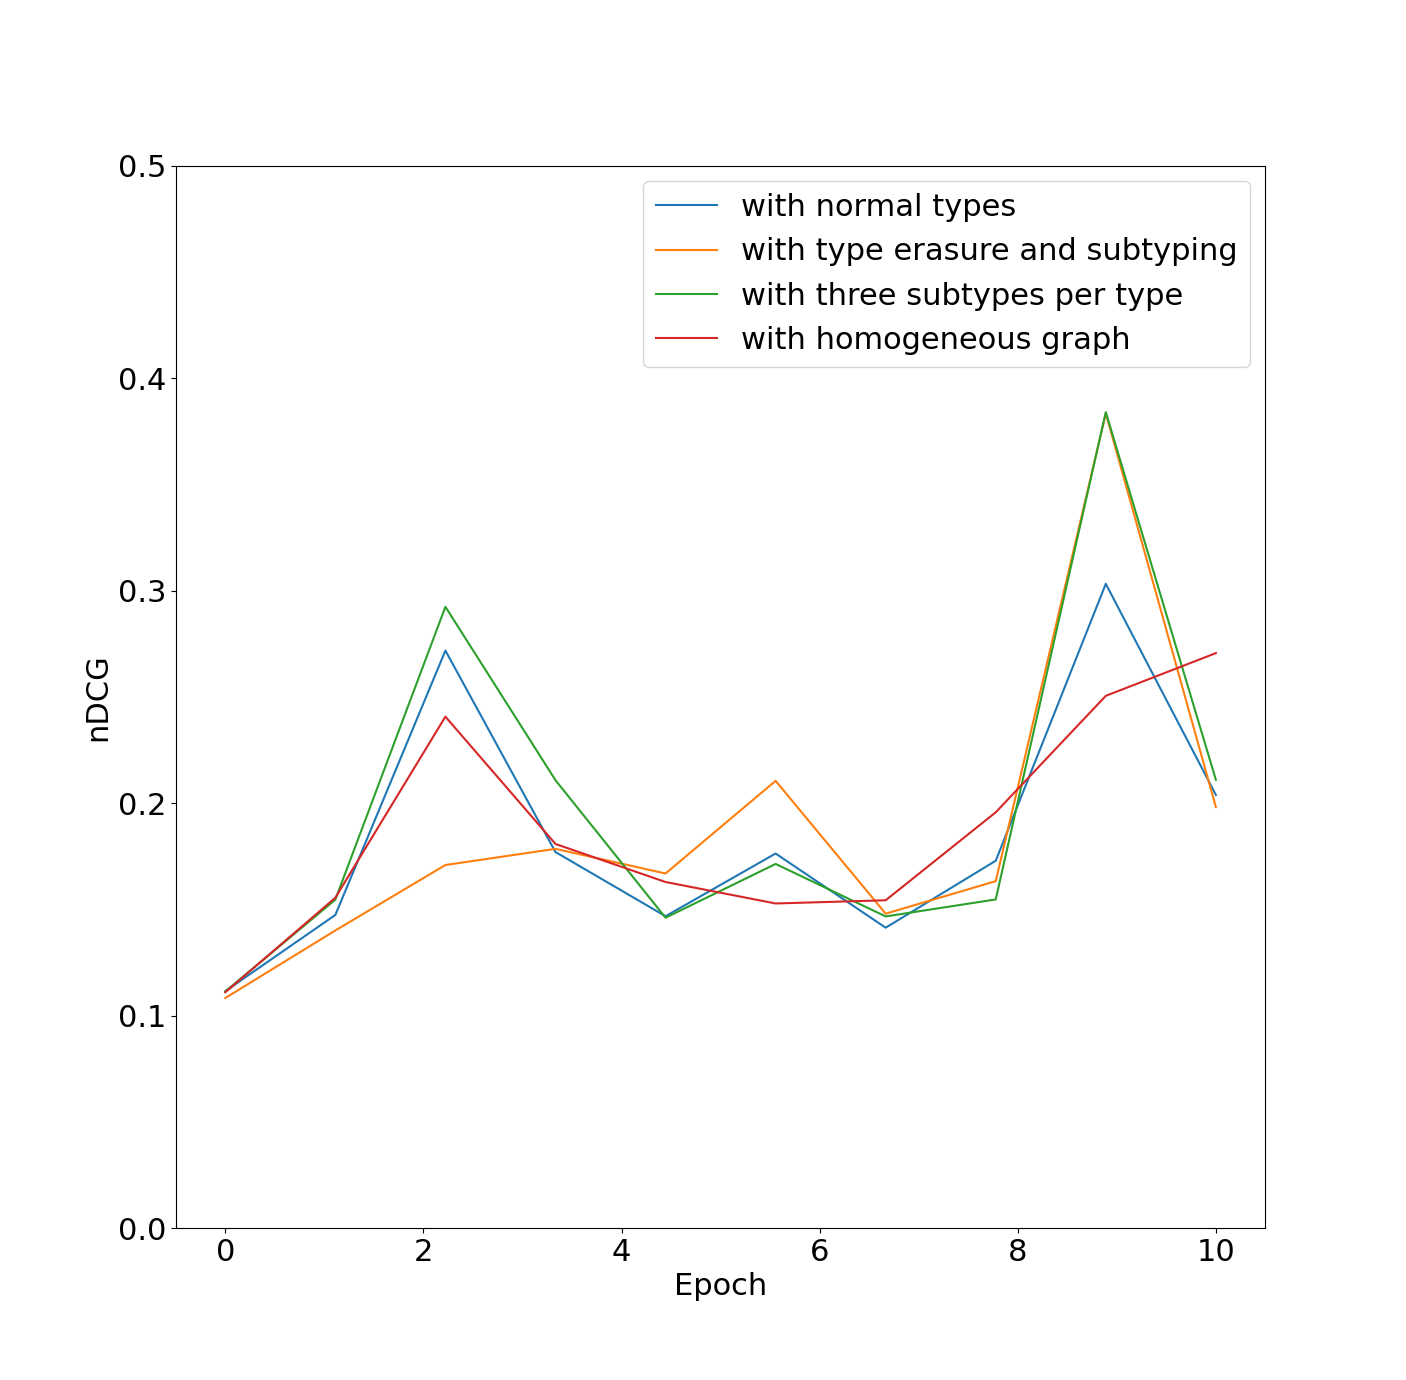
\includegraphics[width=.9\linewidth]{./images/proposal-plot.png}
\caption{}
\label{fig:results} % TODO this gets counted as figure 2 instead of 1 - probably because of the logos on the cover
\end{figure}


Figure \ref{fig:results} shows that adding more types consistently outperforms having fewer types.
Adding three subtypes on top of the normal given types produces the best results.
When comparing the five normal types with erasing the types and creating five subtypes ourselves, it is notable that the normal HGT seems better at first, but our subtypes quickly catch up and surpass them.
Completely erasing all type information predictably produces the worst results.

These findings suggest that more type granularisation can successfully improve performance.


\section{Next Steps}

Our next steps are as follows.

\subsection{Dynamically generate subtypes}

In the current prototype, we specify the number of subtypes to generate for each type.
While the results with that are already promising, the automatic generation of a dynamic number of subtypes via the importance calculation detailed above is an important part of our solution, and will make it possible to scale to unknown datasets.

\subsection{Improve Meta-Learning}

The system should be able to quickly accomodate new items from our constantly changing world.
Methods like Model-Agnostic Meta Learning \cite{finn_model-agnostic_2017} can be used to learn parameters that are more easily adaptable.

\subsection{Improve Clustering}

Our current implementation uses a simple agglomerative clustering algorithm.
As a next step in the thesis, we would like to test if more sophisticated clustering algorithms like GSDMM~\cite{yin_gsdmm_2014}
can improve performance.


\subsection{Improve Processing} 

Our current implementation processes subtypes by a simple linear transformation.
As a next step in the thesis, we would like to test if more sophisticated transformations, like variational autoencoders~\cite{kingma_auto-encoding_2022}, can improve performance.



